\documentclass[xcolor=dvipsnames]{beamer}

\usetheme{Madrid}

\usepackage{mpctools}
\usepackage{standalone}

\title{MPC with Casadi/Python}
\date{June 10, 2015}
\author{Michael Risbeck}

\begin{document}

\frame{\titlepage}

%\begin{frame}{Windows Installation}
%    A Windows Python distribution.
%    \begin{itemize}
%        \item Any ``Scientific Python'' should do, but it must include NumPy, SciPy, and matplotlib.
%        \item E.g., Python(x,y): \smallurl{https://code.google.com/p/pythonxy/}
%    \end{itemize}
%    
%    \medskip
%    
%    CasADi 2.2.0:
%    \begin{itemize}
%        \item Check dependencies from \smallurl{https://github.com/casadi/casadi/wiki/BinaryInstallationWindows}
%        \item Download from \smallurl{http://sourceforge.net/projects/casadi/files/CasADi/}
%        \item Install as you would normal Windows programs
%    \end{itemize}
%    
%    \medskip
%    
%    Our Python package
%    \begin{itemize}
%        \item Download Mercurial repo: \smallurl{https://hg.cae.wisc.edu/hg/mpc-tools-casadi}
%        \item Download \texttt{.zip} file on the left.
%    \end{itemize}
%\end{frame}
%
%\begin{frame}[fragile]{Ubuntu/Debian Installation}
%    Python, NumPy, SciPy, matplotlib
%    \begin{itemize}
%        \item E.g., with Spyder (an IDE): \lstinline[style=shell]@sudo apt-get install spyder@
%    \end{itemize}
%    
%    \medskip
%    
%    CasADi 2.2.0:
%    \begin{itemize}
%        \item Check dependencies from \smallurl{https://github.com/casadi/casadi/wiki/Binaryinstallationlinux}
%        \item Download from \smallurl{http://sourceforge.net/projects/casadi/files/CasADi/}
%        \item Install: \lstinline[style=shell]@dpkg -i <filename>.deb@
%    \end{itemize}
%    
%    \medskip
%    
%    Our python modules
%    \begin{itemize}
%        \item Clone Mercurial repo: \lstinline[style=shell]!hg clone https://hg.cae.wisc.edu/hg/mpc-tools-casadi!
%        \item Or, download a copy from \smallurl{https://hg.cae.wisc.edu/hg/mpc-tools-casadi}
%    \end{itemize}
%\end{frame}
%
%\begin{frame}{Mac Installation (Difficult)}
%    Python, NumPy, SciPy, matplotlib
%    \begin{itemize}
%        \item E.g., via Homebrew: \lstinline[style=shell]!brew install python!
%        \item Packages via \texttt{pip}: \lstinline[style=shell]!pip install ipython matplotlib numpy scipy
%        !
%    \end{itemize}
%    
%    \medskip
%    
%    CasADi 2.2.0
%    \begin{itemize}
%        \item You'll have to build from sources.
%        \item See \smallurl{https://github.com/casadi/casadi/wiki/InstallationMac} for details.
%        \item We can only provide minimal support for this option.
%    \end{itemize}
%    
%    \medskip
%    
%    Our Python package
%    \begin{itemize}
%        \item Download Mercurial repo: \smallurl{https://hg.cae.wisc.edu/hg/mpc-tools-casadi}
%        \item Download \texttt{.zip} file on the left.
%    \end{itemize}
%\end{frame}

\documentclass[xcolor=dvipsnames]{beamer}

\usepackage{mpctools}
\usepackage{hyperref}

\setbeamertemplate{navigation symbols}{}
\newcommand{\clickurl}[1]{\href{#1}{\textcolor{blue}{\smallurl{#1}}}}

\begin{document}
%
\begin{frame}[allowframebreaks]{Installation}
    Install a scientific Python 2.7 distribution
    \begin{itemize}
        \item Any ``Scientific Python'' should do, but it must include NumPy, SciPy, matplotlib, and Tkinter.
        \item Be sure to choose 2.7 and not 3.x
        \item Spyder (a Python IDE) is very helpful but not required.
        \item See the \hyperlink{scientificpython}{\textcolor{blue}{Scientific Python Options}} slides for some good choices
    \end{itemize}
    
    \medskip
    
    Download our \texttt{mpctools} Python package
    \begin{itemize}
        \item Download zipped package: \clickurl{https://bitbucket.org/rawlings-group/mpc-tools-casadi}
        \begin{itemize}
            \item Click ``Downloads'' (cloud icon on left)
            \item Choose \texttt{mpc-tools-casadi.zip}
        \end{itemize}
        \item Unzip to a convenient location.
    \end{itemize}
    
    \framebreak
    
    Download \casadi{} (Version $\ge$3.0)
    \begin{itemize}
        \item Windows/Linux/Mac zip file available at \clickurl{http://files.casadi.org}
            \begin{itemize}
                \item Choose 3.1.1, pick OS, and download \texttt{casadi-py27-*.zip}
            \end{itemize}
        \item Unzip \texttt{casadi}, to the \texttt{mpc-tools-casadi} folder from the previous step.
    \end{itemize}
    
    \medskip
    
    Optional: Add CasADi and \texttt{mpctools} to your Python path
    \begin{itemize}
        \item Open a Python interpreter (run \lstinline[style=shell]!python! from a terminal/command prompt)
        \item Run the commands \lstinline[style=python]!import site; print site.getusersitepackages()! to see where your user site packages are stored
        \item Move the \texttt{casadi} and \texttt{mpctools} folders to that location.
        \begin{itemize}
            \item You should make the folders if they do not already exist
        \end{itemize}
    \end{itemize}
\end{frame}

\begin{frame}[allowframebreaks]{Scientific Python Options}
    \label{scientificpython}
    Anaconda (Linux, Windows, Mac)
    \begin{itemize}
        \item Download from \clickurl{https://www.continuum.io/downloads}
        \item Perhaps a bit bloated (contains packages we do not need)
        \item Typically the easiest version to work with.
    \end{itemize}
    
    \medskip
    
    APT (Ubuntu/Debian)
    \begin{itemize}
        \item Use \lstinline[style=shell]@sudo apt-get install spyder@ to get Spyder and all dependencies.
        \item Includes \texttt{python-numpy}, \texttt{python-scipy}, \texttt{python-matplotlib}, and \texttt{python-tk}.
    \end{itemize}
    
    \framebreak
    
    Miniconda (Linux, Windows, Mac)
    \begin{itemize}
        \item Smaller version of Anaconda
        \item Download from \clickurl{http://conda.pydata.org/miniconda.html}
        \item After install, need to install additional components
        \begin{itemize}
            \item Packages: \lstinline[style=shell]@conda install numpy scipy matplotlib tk@
            \item IDE: \lstinline[style=shell]@conda install spyder@
            \item Both commands should be entered in a terminal/command prompt
        \end{itemize}
    \end{itemize}
\end{frame}

\begin{frame}{Making Sure Everything Works}
    First, open a Python interpreter\footnote{Open a command prompt/terminal in the \smallurl{mpc-tools-casadi} folder and enter \lstinline[style=shell]!python!} and run \lstinline[style=python]!import casadi, mpctools!.
    \begin{itemize}
        \item If this doesn't work, make sure your CasADi folder shows up in \lstinline[style=python]!import sys; print sys.path!.
        \item If you have multiple Python distributions on your machine, don't (or at least make sure you're using the one you think you are).
        \item Make sure you are using Python 2.7 (not 3.x).
    \end{itemize}
    
    \medskip
    
    Then, try to run the examples in \smallurl{mpc-tools-casadi}.
    \begin{itemize}
        \item In the Python interpreter, use \lstinline[style=python]!execfile("filename.py")!.
        \item \smallurl{runall.py} will run everything and tell you if there are errors, but you won't see any plots.
    \end{itemize}
\end{frame}

\begin{frame}{Path Considerations}
    Unless you perform the optional step, \texttt{casadi} and \texttt{mpctools} are only accessible locally.
    \begin{itemize}
        \item Avoids cluttering Python system paths
        \item Doesn't need admin access
        \item To update, simply delete folders and re-download
        \item Python interpreter (or IDE) must be started from this folder
    \end{itemize}
    
    \medskip
    
    If you preform the optional step, \texttt{casadi} and \texttt{mpctools} will be accessible everywhere on your machine.
    \begin{itemize}
        \item Any Python interpreter can load the packages
        \item May be difficult to keep track of versions
        \item A local install will override a global install in the local directory
    \end{itemize}
\end{frame}

% Need this macro to split link across two lines.
\newcommand{\winsixtyfour}[1]{\href{https://sourceforge.net/projects/casadi/files/CasADi/commits/de2f632/windows/}{\textcolor{blue}{\footnotesize \texttt{#1}}}}
\begin{frame}[label=specialnotes]{Special Notes}
    The CasADi version you download must match the bitness of your Python installation (i.e., 32 vs. 64 bit).
    \begin{itemize}
        \item For 32 bit: \texttt{casadi-py27-np1.9.1-v3.1.1.zip}
        \item For 64 bit: \texttt{casadi-py27-np1.9.1-v3.1.1-64bit.zip}
        \item You can check Python bitness in an interpreter with \lstinline[style=python]!import sys; print 64 if sys.maxsize > 2**32 else 32!
    \end{itemize}
\end{frame}

\begin{frame}{Software Relationships}
    \centering
    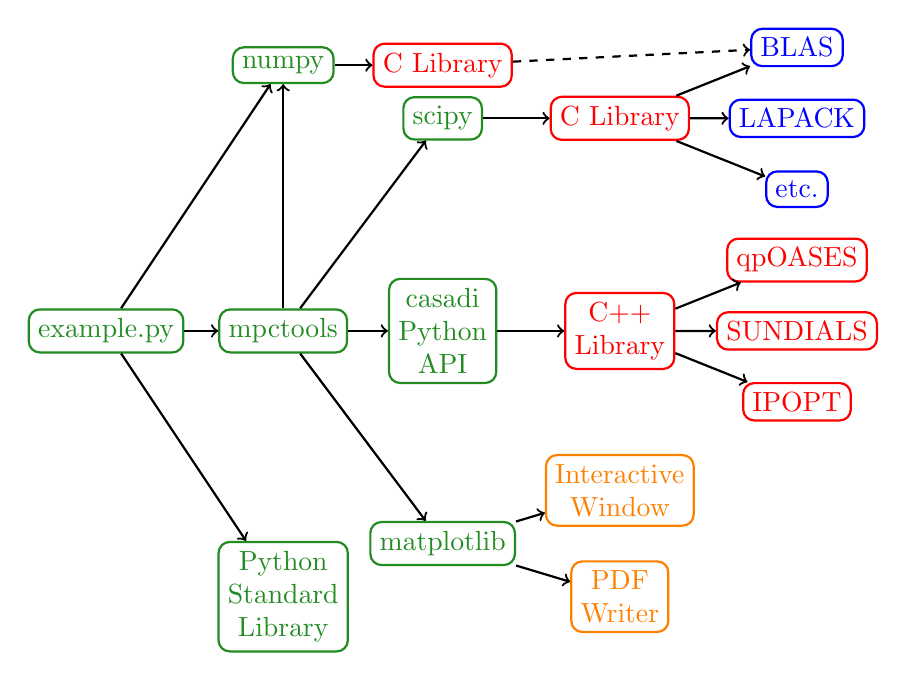
\begin{tikzpicture}
        [
            grow=right,
            code/.style={rectangle,rounded corners,align=center,thick},
            python/.style={code,draw=ForestGreen,text=ForestGreen},
            clib/.style={code,draw=Red,text=Red},
            fortran/.style={code,draw=Blue,text=Blue},
            backend/.style={code,draw=orange,text=orange},
            level 1/.style={level distance=2.5cm,sibling distance=3.75cm},
            level 2/.style={level distance=2.25cm,sibling distance=3cm},
            level 3/.style={level distance=2.5cm,sibling distance=1.5cm},
            level 4/.style={level distance=2.5cm,sibling distance=1cm},
            level 5/.style={level distance=2.5cm,sibling distance=1cm},
            arw/.style={->,thick},
            scale=.9,
        ]
        \draw (0,0) node[python] {example.py}
        child
        {
            node[python] {Python\\Standard\\Library}
            edge from parent [arw]
        }
        child
        {
            node[python] (mpc) {mpctools}
            child
            {
                node[python] (matplotlib) {matplotlib}
                child
                {
                    node [backend] {PDF\\Writer}
                    edge from parent [arw]
                }
                child
                {
                    node [backend] {Interactive\\Window}
                    edge from parent [arw]
                }
                edge from parent [arw]
            }
            child
            {
                node[python] (casadipy) {casadi\\Python\\API}
                child
                {
                    node[clib] {C++\\Library}
                    child
                    {
                        node[clib] {IPOPT}
                        edge from parent [arw]
                    }
                    child
                    {
                        node[clib] {SUNDIALS}
                        edge from parent [arw]
                    }
                    child
                    {
                        node[clib] {qpOASES}
                        edge from parent [arw]
                    }
                    edge from parent [arw]
                }
                edge from parent [arw]
            }
            child
            {
                node[python] (scipy) {scipy}
                child
                {
                    node[clib] {C Library}
                    child
                    {
                        node[fortran] {etc.}
                        edge from parent [arw]
                    }
                    child
                    {
                        node[fortran] {LAPACK}
                        edge from parent [arw]
                    }
                    child
                    {
                        node[fortran] (blas) {BLAS}
                        edge from parent [arw]
                    }
                    edge from parent [arw]
                }
                edge from parent [arw]
            }
            edge from parent [arw]
        }
        child
        {
            node[python] (numpy) {numpy}
            child
            {
                node[clib] (numpylib) {C Library}
                edge from parent [arw]
            }
            edge from parent [arw]
        };
        \draw[arw] (mpc) -- (numpy);
        \draw[arw,dashed] (numpylib) -- (blas);
    \end{tikzpicture}
\end{frame}
%
%
\end{document}

\begin{frame}{What's in \texttt{mpc-tools-casadi}?}
    A Python package: \texttt{mpctools}.
    \begin{itemize}
        \item You should put the \texttt{mpctools} folder somewhere on your Python path.
        \item In Python, use \lstinline[style=python]!import sys; print sys.path! to see what folders are on your path.
    \end{itemize}
    
    \medskip
    
    A cheatsheet (in the \texttt{doc} folder).
    \begin{itemize}
        \item Should get you started writing your own code.
        \item Compares plain CasADi vs. CasADi + \texttt{mpctools}.
    \end{itemize}
    
    \medskip
    
    A bunch of example files.
    \begin{itemize}
        \item \texttt{nmpcexample.py}: Example of linear vs. nonlinear MPC.
        \item \texttt{cstr\_startup.py}: startup and a setpoint change (with no disturbances) for the CSTR system from Example 1.11.
        \item \texttt{nmheexample.py}: NMHE (with EKF to update prior) for a batch reactor (See Example 4.27 in the textbook).
    \end{itemize}
\end{frame}

\begin{frame}{Making Sure Everything Works}
    To check that everything works, try to run the examples in \texttt{mpc-tools-casadi}.
    \begin{itemize}
        \item \texttt{runall.py} will run everything and tell you if there are errors.
        \item You won't see any output, however.
    \end{itemize}
    
    \medskip
    
    If this fails, open a Python interpreter and try \texttt{import casadi}.
    \begin{itemize}
        \item If this doesn't work, then CasADi must have installed to the wrong Python distribution.
        \item If you have multiple Python distributions on your machine, don't (or at least make sure you're using the one you think you are).
        \item Make sure you are using Python 2.7 (not 3.x).
    \end{itemize}
\end{frame}


%\begin{frame}[fragile]{Developers}
%
%A few extra steps if you want to be able to push changes:
%
%\begin{itemize}
%    \item Get Jim to authorize you
%    \item Go to \smallurl{https://my.cae.wisc.edu/}
%    \item Web Tools $\rightarrow$ Repositories
%    \item Set Alternate Repository Passwords
%    \item Add lines to \smallurl{.hg/hgrc}:
%\end{itemize}
%
%\begin{lstlisting}[style=shell]
%    [auth]
%    .prefix = hg.cae.wisc.edu/hg
%    .username = <username>
%    .password = <password>
%\end{lstlisting}
%
%\end{frame}


\begin{frame}{Why did we write this code?}

\begin{itemize}
    \item We plan to solve nonlinear MPC problems.
    \item CasADi is more robust than our \texttt{mpc-tools}
    \item However, setting up an MPC problem in CasADi takes a fair bit of code
    \item Everyone copy/pasting their own code is bad.
    \item A simpler interface means we (and others) can save a lot of time.
\end{itemize}

\end{frame}

\begin{frame}[fragile]{From official CasADi Examples}

\begin{columns}
    \begin{column}{.75\textwidth}
        
\begin{lstlisting}[style=python,basicstyle=\ttfamily\fontsize{6}{8}\selectfont]
# For all collocation points: eq 10.4 or 10.17 in Biegler's book
# Construct Lagrange polynomials to get the polynomial basis at
# the collocation point
for j in range(deg+1):
    L = 1
    for j2 in range(deg+1):
        if j2 != j:
            L *= (tau-tau_root[j2])/(tau_root[j]-tau_root[j2])
    
    lfcn = SXFunction([tau],[L])
    lfcn.init()
    # Evaluate the polynomial at the final time to get the
    # coefficients of the continuity equation
    lfcn.setInput(1.0)
    lfcn.evaluate()
    D[j] = lfcn.getOutput()
    
    # Evaluate the time derivative of the polynomial at all
    #collocation points to get the coefficients of the
    #continuity equation
    tfcn = lfcn.tangent()
    tfcn.init()
    for j2 in range(deg+1):
        tfcn.setInput(tau_root[j2])
        tfcn.evaluate()
        C[j][j2] = tfcn.getOutput()
\end{lstlisting}
    \end{column}
    \begin{column}{.25\textwidth}
        We don't want everyone writing this themselves!
    \end{column}
\end{columns}

\end{frame}

\begin{frame}[fragile]{Python Basics}
    For our purposes Python+Numpy isn't that much different from Octave/\textsc{Matlab}.
    
    \begin{center}
        \begin{tabular}{ll}
            \toprule
            Octave/\textsc{Matlab} & Python+Numpy \\
            \midrule
            \lstinline[style=matlab]!A = zeros(3,2);! & \lstinline[style=python]!A = np.zeros((3,2))! \\
            \lstinline[style=matlab]!x = ones(2,1); %  2D.! & \lstinline[style=python]!x = np.ones((2,)) #  1D.! \\
            \lstinline[style=matlab]!y = A*x;! & \lstinline[style=python]!y = A.dot(x)! \\
            \lstinline[style=matlab]!z = y.^2; %  Elementwise.! & \lstinline[style=python]!z = y**2 #  Elementwise.! \\
            \lstinline[style=matlab]!A(1,1) = 2; %  One-based.! & \lstinline[style=python]!A[0,0] = 2 #  Zero-based.! \\
            \lstinline[style=matlab]!A(2,:) = [3,4];! & \lstinline[style=python]!A[1,:] = np.array([3,4])! \\
            \lstinline[style=matlab]!s = struct('field',1);! & \lstinline[style=python]!s = {"field"  : 1}! \\
            \lstinline[style=matlab]!disp(s.field);! & \lstinline[style=python]!print s["field"]! \\
            \bottomrule
        \end{tabular}
    \end{center}
    
\end{frame}


\begin{frame}{General Tips}
    \begin{itemize}
        \item Remember that indexing is 0-based.
        \item Use NumPy's \texttt{array} instead of \texttt{matrix}.
        \begin{itemize}
            \item Despite what Octave/\textsc{Matlab} says, everything is \emph{not} a matrix of doubles
            \item Have to use \texttt{A.dot(x)} instead of \texttt{A*x}
            \item However, indexing is MUCH easier with arrays
        \end{itemize}
        \item Use \texttt{bmat([[A,B],[C,D]]).A} to assemble matrices from blocks.
        \begin{itemize}
            \item Equivalent to \texttt{[A, B; C, D]} in Octave/\textsc{Matlab}
            \item Trailing \texttt{.A} casts back to \texttt{array} type from \texttt{matrix}
        \end{itemize}
        \item Use \texttt{scipy.linalg.solve(A,b)} to compute $A^{-1}b$.
    \end{itemize}
\end{frame}

\begin{frame}[fragile]{System Model}

Start by defining the system model as a Python function.

\begin{lstlisting}[style=python]
def ode(x,u,d):
    # Grab the states, controls, and disturbance.
    [c, T, h] = x[:Nx]
    [Tc, F] = u[:Nu]
    [F0] = d[:Nd]
    
    # Now create the right-hand side function of the ODE.
    rate = k0*c*np.exp(-E/T)
    
    dxdt = [
        F0*(c0 - c)/(np.pi*r**2*h) - rate,
        F0*(T0 - T)/(np.pi*r**2*h)
        - dH/(rho*Cp)*rate
        + 2*U/(r*rho*Cp)*(Tc - T),
        (F0 - F)/(np.pi*r**2)
    ]
    
    return np.array(dxdt)
\end{lstlisting}
\end{frame}

\begin{frame}[fragile]{System Simulation}

The nonlinear system can be simulated using CasADi \texttt{integrator} objects with a convenient wrapper.
    
\begin{lstlisting}[style=python]
# Turn into casadi function and simulator.
ode_casadi = mpc.getCasadiFunc(ode,
    [Nx,Nu,Nd],["x","u","d"],funcname="ode")
cstr = mpc.DiscreteSimulator(ode, Delta, [Nx,Nu,Nd], ["x","u","d"])

# Simulate with nonlinear model.
x[n+1,:] = cstr.sim(x[n,:] + xs, u[n,:] + us, d[n,:] + ds) - xs
\end{lstlisting}

\end{frame}

\begin{frame}[fragile]{Calls to LQR and LQE}

\vspace{-10pt}
The functions \texttt{dlqr} and \texttt{dlqe} are also provided in \texttt{mpc-tools-casadi}.
\begin{columns}[T]

\begin{column}[T]{0.49\textwidth}
\begin{block}{Octave/\textsc{Matlab}}

\begin{lstlisting}[style=matlab]
% Get LQR.
[K, Pi] = dlqr(A, B, Q, R);

% Get Kalman filter.
[L, M, P] = dlqe(Aaug, ...
    eye(naug), Caug, Qw, Rv);
Lx = L(1:n,:);
Ld = L(n+1:end,:);

\end{lstlisting}

\end{block}
\end{column}

\begin{column}[T]{0.49\textwidth}
\begin{block}{CasADi/Python}

\begin{lstlisting}[style=python]
# Get LQR.
[K, Pi] = mpc.util.dlqr(A,B,Q,R)

# Get Kalman filter.
[L, P] = mpc.util.dlqe(Aaug,
    Caug, Qw, Rv)
Lx = L[:Nx,:]
Ld = L[Nx:,:]        


\end{lstlisting}

\end{block}
\end{column}

\end{columns}     

\end{frame}

\begin{frame}[fragile]{Controller Simulation}

\vspace{-1.5em}
\begin{columns}[T]

\begin{column}[T]{0.45\textwidth}
\begin{block}{Octave/\textsc{Matlab}}
\vspace*{-.75em}
\begin{lstlisting}[style=matlab,basicstyle=\ttfamily\fontsize{5pt}{6}\selectfont]
for i = 1:ntimes
  % Take plant measurement.
  y(:,i) = C*x(:,i) + v(:,i);
  
  % Update state estimate with measurement.
  ey = y(:,i) - C*xhatm(:,i) -Cd*dhatm(:,i);
  xhat(:,i) = xhatm(:,i) + Lx*ey;
  dhat(:,i) = dhatm(:,i) + Ld*ey; 
  
  % Steady-state target.
  H  = [1 0 0; 0 0 1];
  G = [eye(n)-A, -B; H*C, zeros(size(H,1), m)];
  qs = G\[Bd*dhat(:,i); ...
      H*(target.yset-Cd*dhat(:,i))];
  xss = qs(1:n); 
  uss = qs(n+1:end);
  
  % Regulator.
  u(:,i) = K*(xhat(:,i) - xss) + uss; 
  if (i == ntimes) break; end 
  
  % Simulate with nonlinear model.
  t = [time(i); mean(time(i:i+1)); time(i+1)];
  z0 = x(:,i) + zs;   F0 = p(:,i) + Fs;
  Tc = u(1,i) + Tcs;  F  = u(2,i) + Fs;
  [tout, z] = ode15s(@massenbal, t, z0, opts);
  x(:,i+1) = z(end,:)' - zs;
  
  % Advance state estimate.
  xhatm(:,i+1) = A*xhat(:,i) ...
      + Bd*dhat(:,i) + B*u(:,i);
  dhatm(:,i+1) = dhat(:,i);
end
\end{lstlisting}
\vspace{-.5em}
\end{block}
\end{column}

\begin{column}[T]{0.45\textwidth}
\begin{block}{Python+Numpy \vphantom{/}}
\vspace*{-.75em}
\begin{lstlisting}[style=python,basicstyle=\ttfamily\fontsize{5pt}{6}\selectfont]
for n in range(Nsim + 1):
    # Take plant measurement.
    y[n,:] = C.dot(x[n,:]) + v[n,:]
    
    # Update state estimate with measurement.
    err[n,:] = (y[n,:] - C.dot(xhatm[n,:])
        - Cd.dot(dhatm[n,:]))
    xhat[n,:] = xhatm[n,:] + Lx.dot(err[n,:])
    dhat[n,:] = dhatm[n,:] + Ld.dot(err[n,:])
    
    # Make sure we aren't at the last timestep.
    if n == Nsim: break

    # Steady-state target.
    rhs = np.concatenate((Bd.dot(dhat[n,:]),
        H.dot(ysp[n,:] - Cd.dot(dhat[n,:]))))
    qsp = linalg.solve(G,rhs) # i.e. G\rhs.
    xsp = qsp[:Nx]
    usp = qsp[Nx:]
    
    # Regulator.
    u[n,:] = K.dot(xhat[n,:] - xsp) + usp
    
    # Simulate with nonlinear model.
    x[n+1,:] = cstr.sim(x[n,:] + xs,
        u[n,:] + us, d[n,:] + ds) - xs
    
    # Advance state estimate.
    xhatm[n+1,:] = (A.dot(xhat[n,:])
        + Bd.dot(dhat[n,:]) + B.dot(u[n,:]))
    dhatm[n+1,:] = dhat[n,:]
                       
\end{lstlisting}
\vspace{-.5em}
\end{block}
\end{column}

\end{columns}     

\end{frame}

\begin{frame}{Results}

\begin{columns}
    \begin{column}{.475\textwidth}
        \begin{block}{Octave/\textsc{Matlab}}
            \begin{center}
                \includegraphics[width=\textwidth]{cstr_octave.pdf}
            \end{center}
        \end{block}
    \end{column}
    
    \begin{column}{.475\textwidth}
        \begin{block}{Python+Numpy \vphantom{/}}
            \begin{center}
                \includegraphics[width=\textwidth]{cstr_python.pdf}
            \end{center}
        \end{block}
    \end{column}
\end{columns}

\end{frame}


\begin{frame}{What can we do with \texttt{mpc-tools-casadi}?}
    \begin{itemize}
        \item Discrete-time linear MPC
        \item Discrete-time nonlinear MPC
        \begin{itemize}
            \item Explicit models
            \item Runge-Kutta discretization
            \item Collocation
        \end{itemize}
        \item Discrete-time nonlinear MHE
        \begin{itemize}
            \item Explicit models
            \item Runge-Kutta discretization
            \item Collocation
        \end{itemize}
        \item Basic plotting function
        \item Example scripts
        \begin{itemize}
            \item Linear
            \item Solution of linear as nonlinear
            \item Periodic linear
            \item Example 2-8
            \item Simple collocation
            \item Example 1-11
        \end{itemize}
    \end{itemize}
    
\end{frame}

\begin{frame}[fragile,allowframebreaks]{Example Script}

Example script for a simple nonlinear MPC problem.

\begin{lstlisting}[style=python,basicstyle=\ttfamily\fontsize{6pt}{8}\selectfont]
# Control of the Van der Pol oscillator.
import mpctools as mpc
import numpy as np

# Define model and get simulator.
Delta = .5
Nsim = 20
Nx = 2
Nu = 1
def ode(x,u):
    dxdt = [(1 - x[1]*x[1])*x[0] - x[1] + u, x[0]]
    return np.array(dxdt)

# Create a simulator.
vdp = mpc.DiscreteSimulator(ode, Delta, [Nx,Nu], ["x","u"])

# Then get nonlinear casadi functions and a linearization.
ode_casadi = mpc.getCasadiFunc(ode, [Nx,Nu], ["x","u"], funcname="f")
lin = mpc.util.getLinearization(ode_casadi,[0,0],[0],Delta=Delta)

# Also discretize using RK4.
ode_rk4_casadi = mpc.getCasadiFunc(ode_rk4, [Nx,Nu], ["x","u"], funcname="F",
                                   rk4=True, Delta=Delta, M=1)

# Define stage cost and terminal weight.
def lfunc(x,u): return mpc.mtimes(x.T,x) + mpc.mtimes(u.T,u)
l = mpc.getCasadiFunc(lfunc, [Nx,Nu], ["x","u"], funcname="l")

def Pffunc(x): return 10*mpc.mtimes(x.T,x)
Pf = mpc.getCasadiFunc(Pffunc, [Nx], ["x"], funcname="Pf")

# Create linear discrete-time model for comparison.
def Ffunc(x,u): return (mpc.mtimes(mpc.util.DMatrix(lin["A"]),x) +
    mpc.mtimes(mpc.util.DMatrix(lin["B"]),u))
F = mpc.getCasadiFunc(Ffunc, [Nx,Nu], ["x","u"], funcname="F")

# Make optimizers.
x0 = np.array([0,1])
Nt = 20
commonargs = dict(
    N={"x":Nx, "u":Nu, "t":Nt},
    verbosity=0,
    l=l,
    x0=x0,
    Pf=Pf,
    lb={"u" : -.75*np.ones((Nsim,Nu))},
    ub={"u" : np.ones((Nsim,Nu))},
    runOptimization=False,
)
solvers = {}
solvers["lmpc"] = mpc.nmpc(f=F,**commonargs)
solvers["nmpc"] = mpc.nmpc(f=ode_rk4_casadi,**commonargs)

# Now simulate.
times = Delta*Nsim*np.linspace(0,1,Nsim+1)
x = {}
u = {}
for method in solvers.keys():
    x[method] = np.zeros((Nsim+1,Nx))
    x[method][0,:] = x0
    u[method] = np.zeros((Nsim,Nu))
    for t in range(Nsim):
        solvers[method].fixvar("x",0,x[method][t,:])
        solvers[method].solve()
        print "%5s %d: %s" % (method,t,solvers[method].stats["status"])
        u[method][t,:] = solvers[method].var["u",0,:]
        x[method][t+1,:] = vdp.sim(x[method][t,:],u[method][t,:])
    fig = mpc.plots.mpcplot(x[method],u[method],times,title=method)
    fig.savefig("vdposcillator_%s.pdf" % (method,))
\end{lstlisting}

\end{frame}

\begin{frame}{Output}

For this problem, nonlinear MPC performs slightly better.
\begin{itemize}
    \item The computation isn't much more time-consuming because of the power of Casadi.
    \item The problem isn't difficult to set up because of \texttt{mpc-tools-casadi}.
\end{itemize}
    
\begin{columns}
    \begin{column}{.475\textwidth}
        \begin{block}{Linear MPC}
            \begin{center}
                \includegraphics[width=\textwidth]{vdposcillator_lmpc.pdf}
            \end{center}
        \end{block}
    \end{column}
    \begin{column}{.475\textwidth}
        \begin{block}{Nonlinear MPC}
            \begin{center}
                \includegraphics[width=\textwidth]{vdposcillator_nmpc.pdf}
            \end{center}
        \end{block}
    \end{column}
\end{columns}
\end{frame}

\begin{frame}{More Complicated Example}

Using \texttt{mpc-tools-casadi}, we can replace the LQR and KF from Example 1.11 with nonlinear MPC and MHE.

\begin{itemize}
    \item \texttt{cstr\_startup.py} shows basic structure and a setpoint change.
    \item \texttt{cstr\_nonlinear.py} shows steady-state target finding and NMHE.
    \item See the cheatsheet for important functions and syntax.
\end{itemize}

\end{frame}

\begin{frame}{\texttt{cstr\_startup.py}}
    
    Here, nonlinear MPC knows to be less aggressive.
    \begin{center}
        \includegraphics[width=.75\textwidth]{cstr_startup.pdf}
     \end{center}
\end{frame}


\begin{frame}{What can't we do yet?}
    \begin{itemize}
        \item True continuous-time formulation
        \begin{itemize}
            \item Time-varying functions not supported
            \item Quadrature for objective function is available via Collocation
            \item DAE systems are possible in principle
        \end{itemize}
        \item Quality guess generation
        \begin{itemize}
            \item Solve sequence of smaller problems
            \item Use as initial guess for large problem
            \item Must do ``by hand''
        \end{itemize}
    \end{itemize}
\end{frame}

%\begin{frame}{Additional Notes}
%
%\begin{itemize}
%    \item We may not be able to write good CasADi code, but we at least want to write good Python code
%    \begin{itemize}
%        \item \smallurl{http://docs.python-guide.org/en/latest/writing/style/}
%        \item \smallurl{https://www.python.org/dev/peps/pep-0008/}
%    \end{itemize}
%    \item NumPy is verbose and takes getting used to, especially if you're using matrices
%    \item Duck-typing makes me nervous, but it's kind of a major paradigm of Python
%    \begin{itemize}
%        \item Lists vs. NumPy vectors
%        \item NumPy matrices vs. arrays
%        \item CasADi \texttt{MX} vs. \texttt{SX}
%    \end{itemize}
%    \item ``Easier to Ask Forgiveness than Permission'' is challenging if you don't know what exceptions might be raised
%    \begin{itemize}
%        \item Takes some getting used to if you've been raised on ``Look Before You Leap'' (common in Octave/\textsc{Matlab})
%        \item A brief discussion: \smallurl{http://code.activestate.com/lists/python-list/337643/}
%    \end{itemize}
%\end{itemize}
%
%\end{frame}

\end{document}
